
\documentclass[12pt,a4paper]{article}
\usepackage[utf8]{inputenc}
\usepackage[T1]{fontenc}
\usepackage[brazil]{babel}
\usepackage{amsmath,amssymb,amsfonts}
\usepackage{graphicx}
\usepackage{float}
\usepackage{hyperref}
\usepackage{geometry}
\usepackage{setspace}
\usepackage{caption}
\usepackage{subcaption}
\usepackage{indentfirst}
\usepackage{xcolor}
\usepackage{minted}
\usemintedstyle{colorful}

\setminted{
    breaklines=true,        % quebra automaticamente linhas longas
    breakanywhere=true,     % permite quebra mesmo sem espaços
    fontsize=\footnotesize, % reduz tamanho da fonte para melhor encaixe
    tabsize=2,              % tamanho das tabulações
    frame=single,           % adiciona uma moldura ao redor do código
    framesep=2mm,           % espaçamento interno entre texto e moldura
    baselinestretch=1.1,    % leve aumento do espaçamento vertical
    bgcolor=white,          % fundo branco (garante contraste com a moldura)
    linenos=false           % números de linha desativados (pode mudar para true)
}


\geometry{a4paper, left=25mm, right=25mm, top=25mm, bottom=25mm}
\onehalfspacing

\begin{document}
\begin{titlepage}
    \begin{center}
        
\includegraphics[width=0.25\textwidth]{EP.jpg}\\[1cm]
        {\Large \textbf{Escola Politécnica da Universidade de São Paulo}}\\[0.2cm]
        {\large Departamento de Engenharia de Computação e Sistemas Digitais}\\[2.0cm]
        {\Huge \textbf{Tarefa 04}}\\[0.4cm]
        {\Large \textbf{Sistemas não lineares e Método de Newton}}\\[2.0cm]
        {\large \textbf{Disciplina:} PTC5725 -- Introdução aos Métodos Espectrais}\\[0.3cm]
        {\large \textbf{Professor:} Osvaldo Guimarães}\\[0.3cm]
        {\large \textbf{Aluno:} Renan de Luca Avila}\\[0.3cm]
        {\large \textbf{Data:} \today}\\[2.5cm]
        \vfill
    \end{center}
\end{titlepage}

\tableofcontents
\newpage

% ---------------- Resumo ----------------
\section*{Resumo}
\addcontentsline{toc}{section}{Resumo}
Este relatório apresenta os enunciados e as resoluções dos Exercícios 1 e 2 da Tarefa 04. 
No Exercício 1, resolvemos um BVP não linear via colocalização de Chebyshev e Newton; no Exercício 2, comparamos Newton--Jacobian (puro/amortecido) e \texttt{fsolve}. 
As análises incluem resíduos, estudo de refinamento (Ex.1), trajetória de Newton e comparação de métodos (Ex.2). 
Os códigos completos de cada exercício estão no Apêndice.

Todo o projeto está disponível no github: \href{https://github.com/stealth-lndrs/PTC5725}{https://github.com/stealth-lndrs/PTC5725}

% ---------------- Enunciados ----------------
\section{Enunciados dos Exercícios}

\subsection{Exercício 1 -- EDO não linear}
Resolver:
\begin{equation}
    y'' = e^{y}, \qquad y(\pm 1) = 1, \qquad x \in [-1, 1].
\end{equation}
Analisar o resíduo
\begin{equation}
    R(x) = y'' - e^{y}
\end{equation}
e a sua derivada \(R'(x)\).\\
\textbf{Fonte:} \textit{Aula 04 -- Introdução aos Métodos Espectrais} (Osvaldo Guimarães, 2025) \cite{guimaraes2025}.

\subsection{Exercício 2 -- Sistema Polinomial (2 variáveis)}
\begin{equation}
\begin{cases}
x^3 + y = 1,\\
y^3 - x = -1.
\end{cases}
\end{equation}
Verificar que \((x,y) = (1,0)\) resolve o sistema.\\
\textbf{Fonte:} \textit{Sistema de ecuaciones no lineales} (Ángel Franco García, 2016) \cite{garcia2016}.

\subsection{Exercício 3 -- Sistema Transcendental (3 variáveis)}
Resolver o sistema de três equações não lineares:
\begin{equation}
\begin{cases}
\sin(xy) + e^{-xz} - 0.9 = 0, \\
z\sqrt{x^2 + y^2} - 6.7 = 0, \\
\tan\!\left(\dfrac{y}{x}\right) + \cos(z) + 3.2 = 0
\end{cases}
\end{equation}
Usar como aproximação inicial: \(x_0=1,\ y_0=2,\ z_0=2\).\\
\textbf{Fonte:} \textit{Sistema de ecuaciones no lineales} (Ángel Franco García, 2016) \cite{garcia2016}.


% ---------------- Ex.1 ----------------
\section{Resolução do Exercício 1}

\subsection{Planejamento.}
Aplicamos colocalização de Chebyshev em \([-1,1]\) para aproximar derivadas via \(D\) e \(D^2\).
Formulamos \(F(y)=D^2y-e^y=0\) e impomos \(y(\pm1)=1\) diretamente nas linhas de fronteira.
Usamos Newton: \(J(y)\Delta y=-F(y)\), com \(J(y)=D^2-\mathrm{diag}(e^y)\), atualizando \(y\leftarrow y+\Delta y\) até \(\|\Delta y\|_\infty<10^{-12}\).

\subsection{Resultados.}
A Figura~\ref{fig:ex1_y_points} mostra \(y(x)\) com pontos; a Figura~\ref{fig:ex1_points_only} exibe apenas os nós.
As Figuras~\ref{fig:ex1_R} e \ref{fig:ex1_Rp} apresentam \(R(x)\) e \(R'(x)\).
A Figura~\ref{fig:ex1_coeff_decay} indica o decaimento espectral de \(|c_k|\).
A Tabela~\ref{tab:ex1_summary} resume métricas; a Tabela~\ref{tab:ex1_refine} mostra o estudo de refinamento.

\begin{figure}[H]
  \centering
  \begin{subfigure}[t]{0.48\textwidth}
    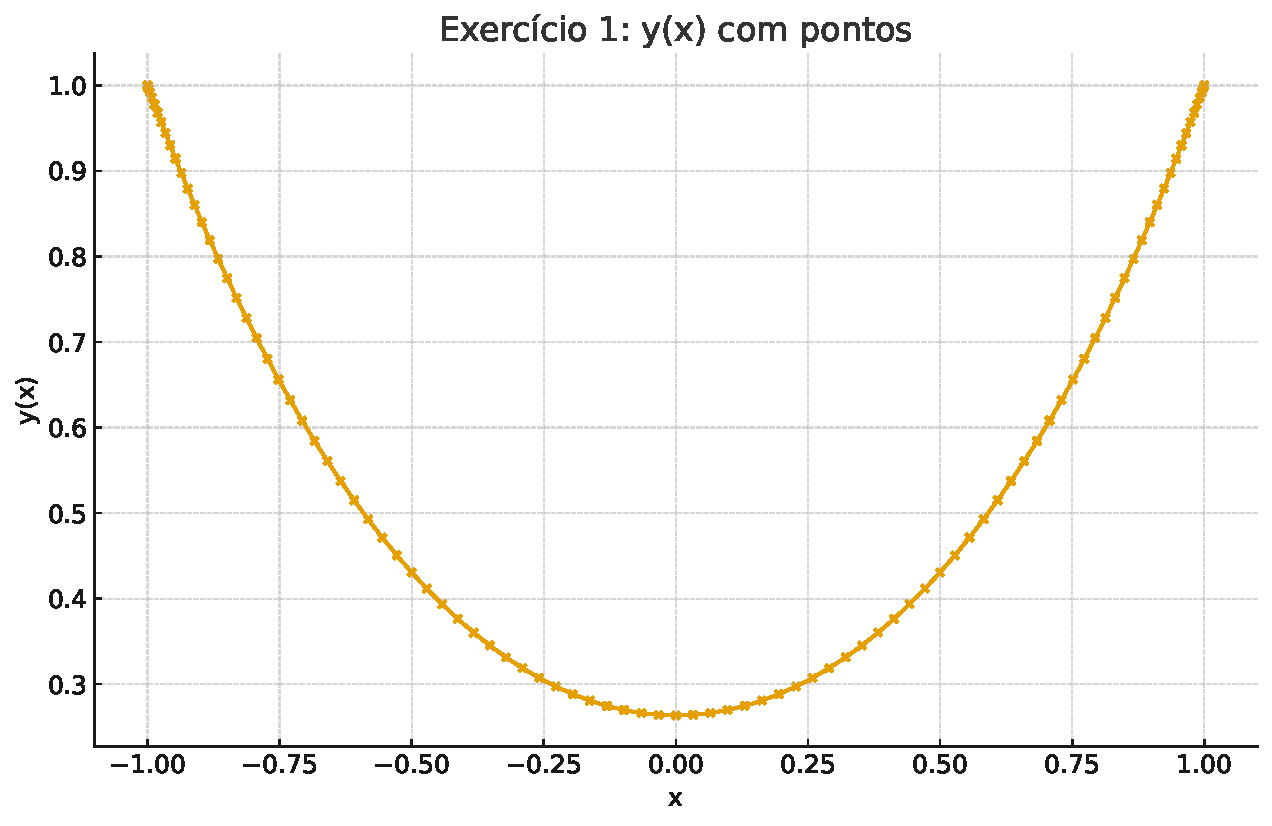
\includegraphics[width=\textwidth]{figures/ex1_solution_with_points.pdf}
    \caption{Solução \(y(x)\) com pontos.}
    \label{fig:ex1_y_points}
  \end{subfigure}\hfill
  \begin{subfigure}[t]{0.48\textwidth}
    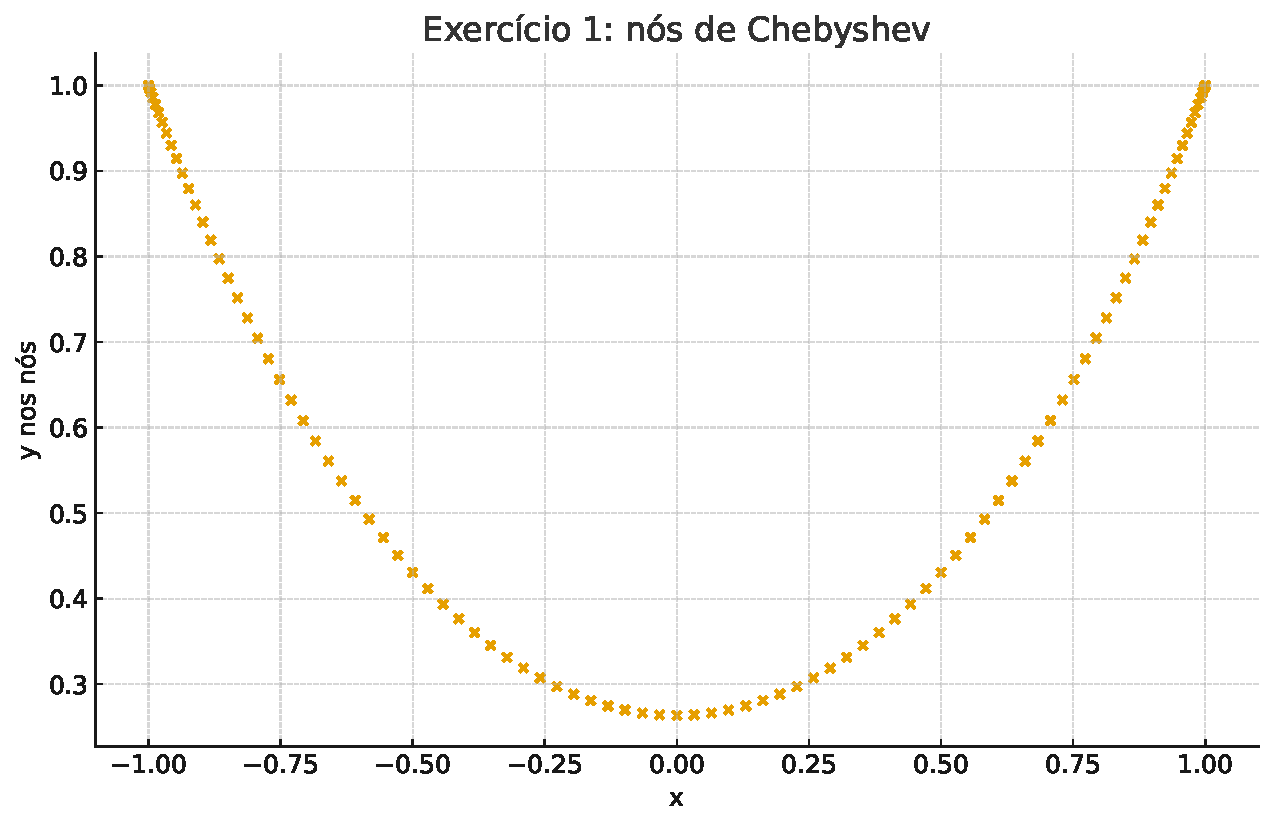
\includegraphics[width=\textwidth]{figures/ex1_points_only.pdf}
    \caption{Nós de Chebyshev.}
    \label{fig:ex1_points_only}
  \end{subfigure}
  \caption{Solução e pontos usados (Ex.1).}
\end{figure}

\begin{figure}[H]
  \centering
  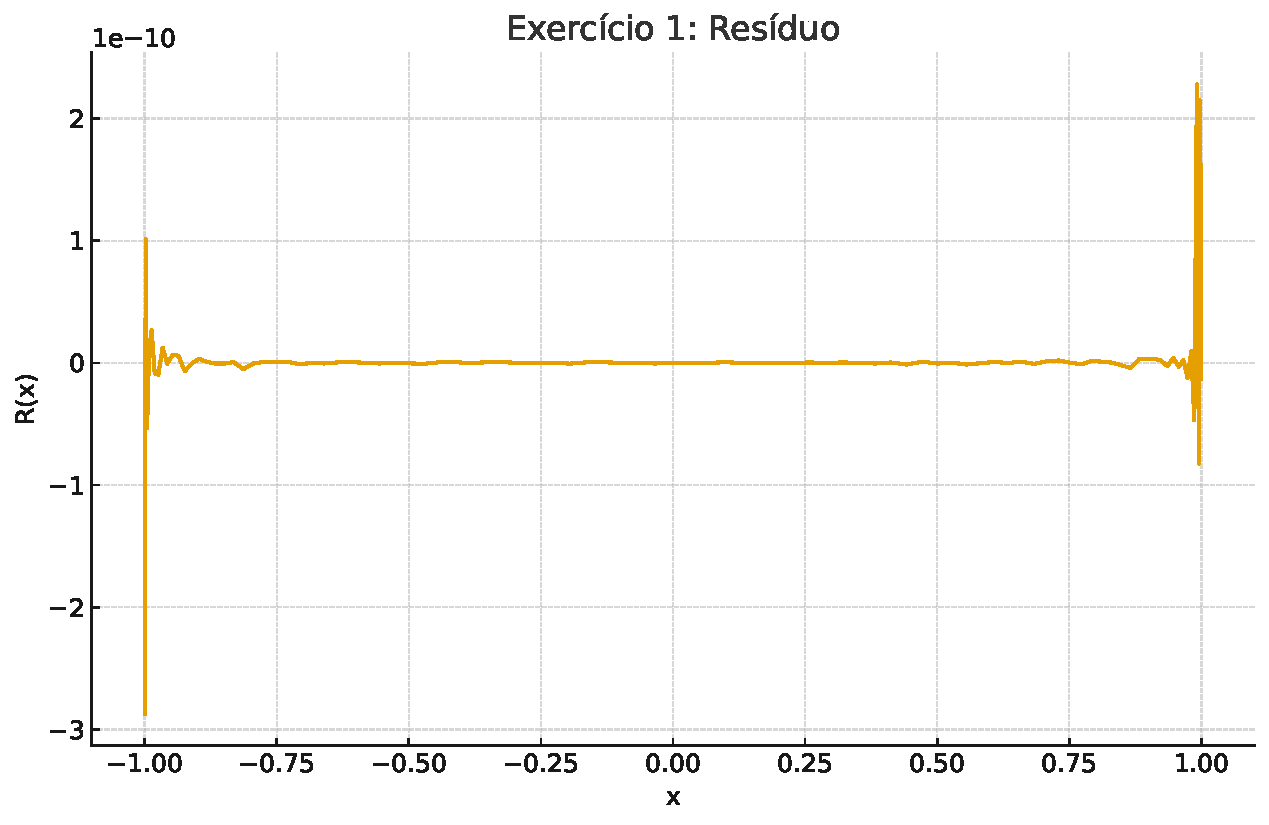
\includegraphics[width=0.8\textwidth]{figures/ex1_residual.pdf}
  \caption{Resíduo \(R(x)=y''-e^y\) (Ex.1).}
  \label{fig:ex1_R}
\end{figure}

\begin{figure}[H]
  \centering
  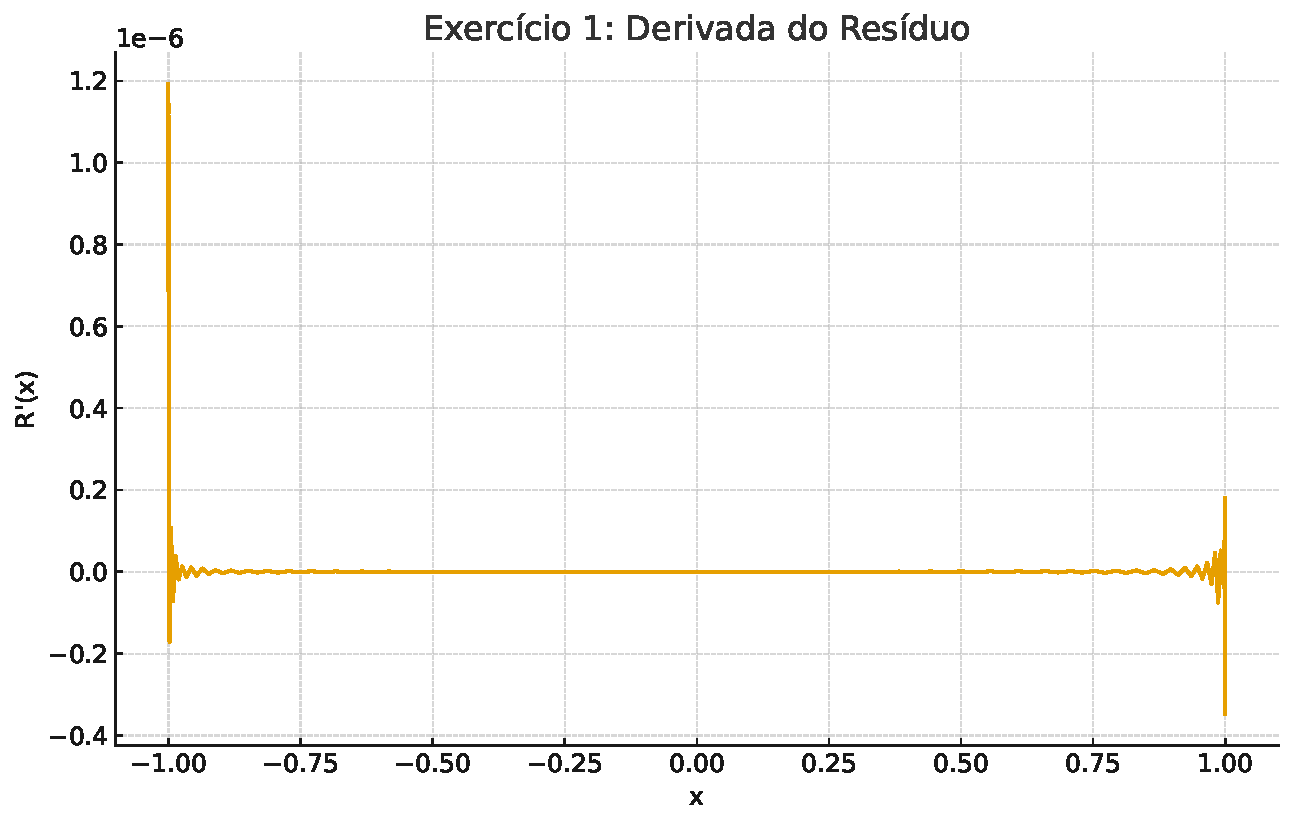
\includegraphics[width=0.8\textwidth]{figures/ex1_residual_prime.pdf}
  \caption{Derivada do resíduo \(R'(x)\) (Ex.1).}
  \label{fig:ex1_Rp}
\end{figure}

\begin{figure}[H]
  \centering
  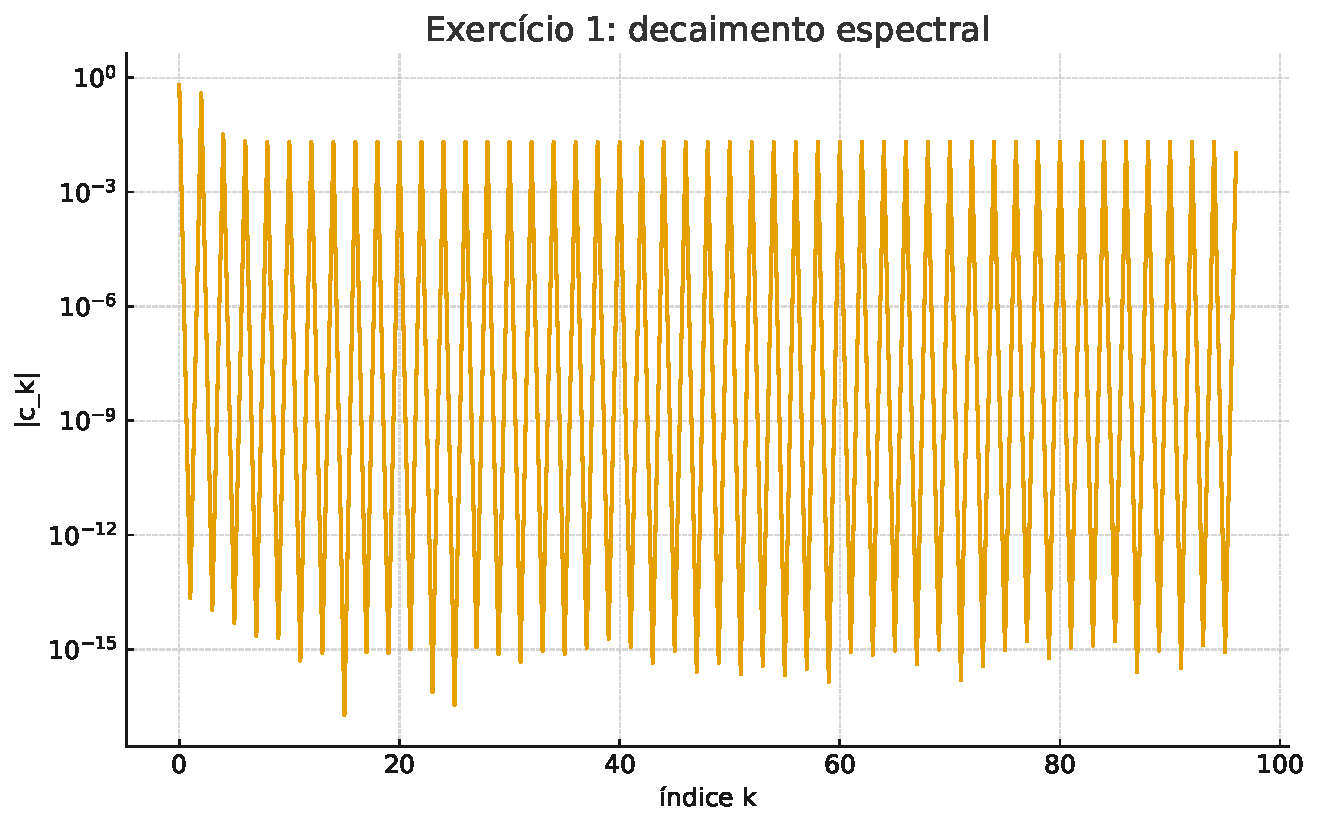
\includegraphics[width=0.8\textwidth]{figures/ex1_coeff_decay.pdf}
  \caption{Decaimento dos coeficientes \(|c_k|\) (Ex.1): eixo x é \(k\); eixo y é \(|c_k|\) (log). Oscilações decorrem de alternância de sinal (função aproximadamente par).}
  \label{fig:ex1_coeff_decay}
\end{figure}

\begin{table}[H]
\centering
\caption{Métricas de convergência (Ex.1).}
\label{tab:ex1_summary}
\begin{tabular}{l r}
\hline
Pontos de Chebyshev \(N{+}1\) & 97 \\
Iterações de Newton & 5 \\
$\|\Delta y\|_{\infty}$ (passo final) & 5.644e-14 \\
$\|R\|_{\infty}$ (resíduo máx. interno) & 2.877e-10 \\
$\|R\|_{2}/\sqrt{N-1}$ (resíduo médio) & 4.644e-11 \\
\hline
\end{tabular}
\end{table}

\begin{table}[H]
\centering
\caption{Estudo de refinamento (Ex.1) em malha fina.}
\label{tab:ex1_refine}
\begin{tabular}{c c c c}
\hline
$N_1$ & $N_2$ & $\|y_{N_2}-y_{N_1}\|_{\infty}$ & $\|y_{N_2}-y_{N_1}\|_{2}/\sqrt{M}$ \\
\hline
48 & 96 & 5.868e-14 & 3.190e-14 \\
\hline
\end{tabular}
\end{table}

\subsection{Conclusão.}
Sem solução analítica, validamos pela combinação: (i) \(R\) e \(R'\) pequenos e suaves; (ii) C.C. satisfeitas; (iii) decaimento rápido de \(|c_k|\); (iv) estabilização entre malhas; (v) passo final de Newton pequeno. Evidências compatíveis com convergência espectral.

\subsection{Implementação}
\label{subsec:ex1-implementacao}

\paragraph{Visão geral do pipeline.}
A solução numérica do BVP
\(y'' = e^{y}\), \(y(\pm1)=1\)
via colocalização de Chebyshev e Newton–Raphson segue os passos:
\begin{enumerate}
    \item Construir os nós de Chebyshev–Lobatto \(x_j=\cos(\pi j/N)\) e a matriz diferencial \(D\); obter \(D^2\).
    \item Montar o sistema não linear discreto \(F(y)=D^2y - e^{y}\).
    \item Impor Dirichlet nas bordas substituindo as linhas de fronteira em \(F\) e no Jacobiano \(J\) (imposição forte das C.C.).
    \item Resolver a correção \(\Delta y\) em \(J(y)\,\Delta y = -F(y)\) e atualizar \(y \leftarrow y + \Delta y\) até convergência (\(\|\Delta y\|_\infty<10^{-12}\)).
    \item Avaliar o resíduo \(R(x)=D^2y-e^{y}\) e sua derivada \(R'(x)=D\,R\); gerar figuras e métricas de convergência.
    \item (Para o estudo de refinamento) projetar soluções em uma malha fina comum via interpolação bariocêntrica e medir diferenças.
\end{enumerate}

\paragraph{Funções principais (arquitetura do código).}
\begin{description}
  \item[\texttt{cheb(N)}] 
  Constrói a matriz diferencial de Chebyshev \(D\in\mathbb{R}^{(N+1)\times(N+1)}\) e os nós \(x\in[-1,1]\) (Chebyshev–Lobatto).
  A construção segue a fórmula fechada clássica (vide Trefethen, \textit{Spectral Methods in MATLAB}). 
  Retorna: \(\,(D, x)\). Usos: derivada de 1ª ordem (\(D\)) e 2ª ordem (\(D^2=D\,D\)).

  \item[\texttt{solve\_bvp\_cheb\_newton(N, tol, maxit)}]
  Resolve o BVP com Newton–Raphson:
  \begin{itemize}
    \item \textbf{Entrada:} número de pontos \(N+1\), tolerância \texttt{tol} (por padrão \(10^{-12}\)) e máximo de iterações \texttt{maxit}.
    \item \textbf{Montagem de \(F\):} \(F(y)=D^2y-e^{y}\). Nas bordas, substitui-se \(F_0 \leftarrow y_0-1\) e \(F_N \leftarrow y_N-1\) (\(y(\pm1)=1\)).
    \item \textbf{Jacobiano:} \(J(y)=D^2-\mathrm{diag}(e^{y})\). Nas bordas, as linhas de \(J\) são substituídas por linhas da identidade (imposição forte das C.C.).
    \item \textbf{Iteração:} resolver \(J\,\Delta y=-F\) e atualizar \(y\) até \(\|\Delta y\|_\infty < \texttt{tol}\).
    \item \textbf{Saída:} \(x\) (nós), \(y\) (solução discreta), \(R=D^2y-e^{y}\) (com \(R_0=R_N=0\) para leitura), \(R'=D\,R\), e um dicionário \texttt{info} com \(\#\)iterações, \(\|\Delta y\|_\infty\), \(\|R\|_\infty\) e \(\|R\|_2/\sqrt{N-1}\).
  \end{itemize}

  \item[\texttt{cheb\_coeffs(y)}]
  Calcula coeficientes \(\{c_k\}\) da expansão de Chebyshev de \(y(x)\) (DCT-I explícita) para análise espectral.
  O \textbf{decaimento exponencial} de \(|c_k|\) indica suavidade e consistência espectral (vide Fig.~\ref{fig:ex1_coeff_decay}).

  \item[\texttt{barycentric\_weights\_cheb(N)} e \texttt{barycentric\_interpolate(...)}]
  (Usadas no estudo de refinamento.) Constroem pesos bariocêntricos e avaliam a interpolação de Lagrange em pontos arbitrários.
  São empregadas para projetar soluções obtidas com malhas diferentes numa \textbf{malha fina comum} e medir \(\|y_{N_2}-y_{N_1}\|\) (Tab.~\ref{tab:ex1_refine}).

  \item[\textit{Rotinas de I/O e figuras}]
  Salvam: amostras \texttt{CSV} (\texttt{tables/ex1\_solution\_samples.csv}), resumo \texttt{JSON} (\texttt{tables/ex1\_summary.json}), 
  e figuras \texttt{PDF} (solução, resíduo \(R\), derivada \(R'\), decaimento \(|c_k|\)).
\end{description}

\paragraph{Escolhas numéricas e critérios.}
Adotamos \(N=96\) pontos de Chebyshev (boa resolução para o problema), tolerância \(\texttt{tol}=10^{-12}\) e \(\texttt{maxit}=50\). 
O critério de parada baseia-se em \(\|\Delta y\|_\infty\). As C.C. são impostas fortemente substituindo linhas (bordas) em \(F\) e \(J\).
Após convergência, avaliamos \(R\) e \(R'\) e conferimos as normas do resíduo no interior do domínio.
Para o estudo de refinamento, projetamos soluções em uma malha fina comum e computamos \(\|\cdot\|_\infty\) e \(\|\cdot\|_2/\sqrt{M}\).

\paragraph{Referência ao código completo.}
O código integral correspondente encontra-se no \textbf{Apêndice} (ver \emph{Exercício 1 — Colocalização de Chebyshev e Método de Newton}), 
onde é \emph{importado} diretamente do arquivo \texttt{code/ex1\_cheb\_newton.py}.


% ---------------- Ex.2 ----------------
\section{Resolução do Exercício 2}

\subsection{Planejamento.}
Para
\[
\begin{cases}
x^3 + y - 1 = 0,\\
y^3 - x + 1 = 0,
\end{cases}
\]
usamos \textbf{Newton--Jacobian} (puro e amortecido por backtracking) e \textbf{\texttt{fsolve}} (SciPy), que emprega abordagens híbridas de região de confiança (e.g., Levenberg--Marquardt/dogleg).

\subsection{Resultados.}
A Figura~\ref{fig:ex2_contours} mostra as curvas $f_1=0$ (contínua) e $f_2=0$ (tracejada); a interseção é \((1,0)\).
A Figura~\ref{fig:ex2_traj} exibe a trajetória típica do Newton amortecido a partir de $(0{,}5,0{,}5)$.
A Tabela~\ref{tab:ex2_methods} resume convergência, iterações e $\|F\|$ para diferentes chutes e métodos.

\begin{figure}[H]
  \centering
  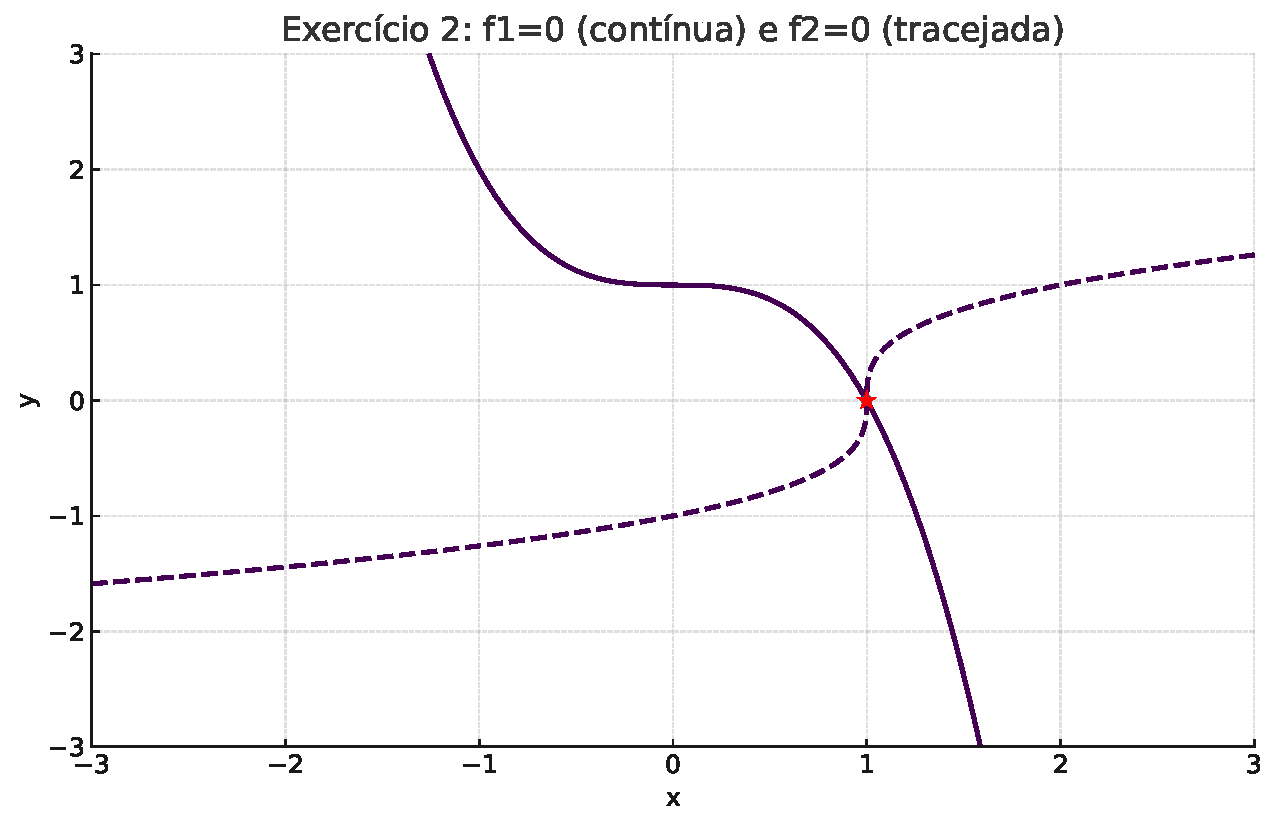
\includegraphics[width=0.8\textwidth]{figures/ex2_contours.pdf}
  \caption{Curvas $f_1=0$ (contínua) e $f_2=0$ (tracejada) e marcação da solução (1,0).}
  \label{fig:ex2_contours}
\end{figure}

\begin{figure}[H]
  \centering
  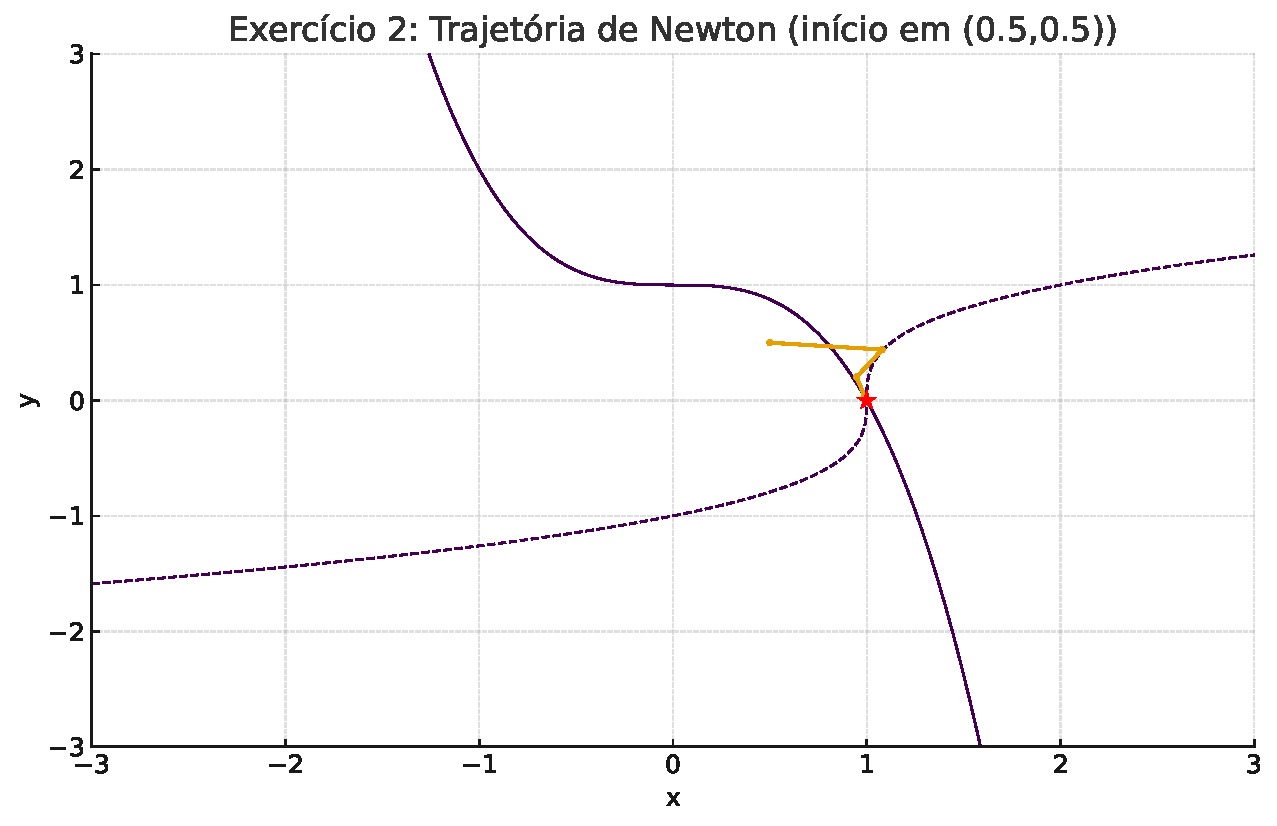
\includegraphics[width=0.75\textwidth]{figures/ex2_newton_trajectory.pdf}
  \caption{Trajetória de Newton amortecido a partir de $(0{,}5,0{,}5)$.}
  \label{fig:ex2_traj}
\end{figure}

\begin{table}[H]
\centering
\caption{Comparação Newton--Jacobian (com/sem amortecimento) e \texttt{fsolve} (Ex.2).}
\label{tab:ex2_methods}
\begin{tabular}{l r r r r r r}
\hline
Método & $x_0$ & $y_0$ & $x$ & $y$ & Convergiu & Iterações \\
\hline
Newton-Jacobian & 0.50 & 0.50 & 1.000000 & -0.000000 & Sim & 7 \\ 
Newton-Jacobian (damped) & 0.50 & 0.50 & 1.000000 & -0.000000 & Sim & 7 \\ 
Newton-Jacobian & 1.50 & 0.50 & 1.000000 & -0.000000 & Sim & 7 \\ 
Newton-Jacobian (damped) & 1.50 & 0.50 & 1.000000 & -0.000000 & Sim & 7 \\ 
Newton-Jacobian & -0.50 & 0.50 & 1.000000 & 0.000000 & Sim & 6 \\ 
Newton-Jacobian (damped) & -0.50 & 0.50 & 1.000000 & 0.000000 & Sim & 6 \\ 
Newton-Jacobian & 2.00 & -1.00 & 1.000000 & -0.000000 & Sim & 7 \\ 
Newton-Jacobian (damped) & 2.00 & -1.00 & 1.000000 & -0.000000 & Sim & 7 \\ 
Newton-Jacobian & -2.00 & 2.00 & 1.000000 & -0.000000 & Sim & 11 \\ 
Newton-Jacobian (damped) & -2.00 & 2.00 & 1.000000 & -0.000000 & Sim & 11 \\ 
fsolve (SciPy) from (0.5,0.5) & 0.50 & 0.50 & 1.000000 & -0.000000 & Sim & 16 \\
\hline
\end{tabular}
\end{table}

\subsection{Conclusão.}
\textbf{Newton puro} é rápido próximo da raiz, porém sensível a chutes ruins e condicionamento do jacobiano; 
\textbf{Newton amortecido} impõe redução de $\|F\|$ a cada passo, ganhando robustez; 
\textbf{\texttt{fsolve}} é geralmente o mais robusto por usar região de confiança, mas pode demandar mais avaliações e custo por iteração.

\subsection{Implementação}
\label{subsec:ex2-implementacao}

\paragraph{Visão geral.}
O código do Exercício~2 implementa a solução do sistema não linear
\[
\begin{cases}
x^3 + y - 1 = 0,\\
y^3 - x + 1 = 0,
\end{cases}
\]
usando duas abordagens: \textbf{Newton–Jacobian} (puro e amortecido) e a alternativa \textbf{\texttt{fsolve}} (SciPy).

O objetivo principal é comparar robustez, velocidade e comportamento de convergência entre os métodos, partindo de diferentes chutes iniciais.

\paragraph{Arquitetura das funções.}
\begin{description}
  \item[\texttt{F(v)}] 
  Define o vetor de funções não lineares \(F(x,y) = [x^3 + y - 1,\; y^3 - x + 1]^T\).
  Essa função é usada em todos os métodos e serve para avaliar o resíduo \(\|F(x_k,y_k)\|\).

  \item[\texttt{J(v)}]
  Retorna o \textbf{Jacobiano exato} do sistema:
  \[
  J(x,y) =
  \begin{bmatrix}
  3x^2 & 1 \\
  -1 & 3y^2
  \end{bmatrix}.
  \]
  A matriz \(J\) lineariza o sistema na vizinhança da solução, permitindo construir o passo de correção de Newton:
  \( J\,\Delta z = -F \).

  \item[\texttt{newton\_jacobian(x0, tol, maxit, damping)}]
  Implementa o método de Newton–Raphson para sistemas de duas variáveis:
  \begin{itemize}
    \item \textbf{Entrada:} chute inicial \(x_0,y_0\), tolerância \(\texttt{tol}\), máximo de iterações \(\texttt{maxit}\) e flag \(\texttt{damping}\) (para amortecimento).
    \item \textbf{Iteração:}
      \begin{enumerate}
        \item Calcula \(F(x_k,y_k)\) e \(J(x_k,y_k)\);
        \item Resolve o sistema linear \(J\,\Delta = -F\);
        \item Atualiza \(x_{k+1},y_{k+1} = x_k,y_k + \alpha\,\Delta\), onde \(\alpha \in (0,1]\) é o fator de amortecimento;
        \item Critério de parada: \(\|F(x_{k+1},y_{k+1})\| < \texttt{tol}\).
      \end{enumerate}
    \item \textbf{Amortecimento (damping):} o parâmetro \(\alpha\) é ajustado por \emph{backtracking} para garantir que o resíduo diminua a cada passo, evitando oscilações ou divergência em chutes distantes da raiz.
    \item \textbf{Saída:} solução aproximada, número de iterações, flag de convergência e histórico.
  \end{itemize}

  \item[\texttt{fsolve(F, x0)}]
  É uma função da biblioteca \texttt{SciPy} que implementa métodos híbridos de região de confiança (Levenberg–Marquardt ou dogleg). 
  Ela combina Newton local (usando \(J\)) com ajustes automáticos de passo e direção, sendo geralmente mais robusta para problemas mal condicionados ou com chutes iniciais ruins.
\end{description}

\paragraph{Diferenças principais entre métodos.}
\begin{itemize}
  \item O \textbf{Newton clássico} possui convergência quadrática próxima da raiz, mas pode divergir com chutes ruins.
  \item O \textbf{Newton amortecido} busca reduzir o resíduo monotonicamente (\(\|F_{k+1}\| < \|F_k\|\)), garantindo maior estabilidade.
  \item O \textbf{\texttt{fsolve}} introduz heurísticas de região de confiança para robustez global, mas requer mais avaliações de \(F\) e \(J\), tornando-se mais caro por iteração.
\end{itemize}

\paragraph{Fluxo geral de execução.}
\begin{enumerate}
  \item Definir os chutes iniciais (vários pontos para avaliar robustez).
  \item Aplicar Newton puro e amortecido em cada chute.
  \item (Opcional) Executar \texttt{fsolve} para comparação.
  \item Registrar resultados (iterações, convergência e solução final) em \texttt{tables/ex2\_newton\_vs\_fsolve\_results.csv}.
  \item Gerar figuras:
    \begin{itemize}
      \item \texttt{ex2\_contours.pdf} — curvas \(f_1=0\) e \(f_2=0\), com pontos de convergência.
      \item \texttt{ex2\_newton\_trajectory.pdf} — trajetória iterativa de Newton a partir de $(0.5,0.5)$.
    \end{itemize}
\end{enumerate}

\paragraph{Critérios numéricos.}
A tolerância de parada é \(\texttt{tol}=10^{-12}\), e o máximo de iterações padrão é 50. 
A convergência é avaliada pela norma Euclidiana do resíduo \(\|F(x_k,y_k)\|_2\).

\paragraph{Referência ao código completo.}
O código integral deste exercício encontra-se no \textbf{Apêndice} (ver \emph{Exercício 2 — Sistema Não Linear: Newton--Jacobian e \texttt{fsolve}}), 
onde é \emph{importado diretamente}.


\subsection*{Discussão: Newton, Newton Amortecido e \texttt{fsolve}}
\begin{itemize}
  \item \textbf{Newton clássico}: convergência quadrática perto da raiz; pode divergir com chutes ruins.
  \item \textbf{Newton amortecido}: introduz fator de passo $\alpha\in(0,1]$ (backtracking) para garantir decréscimo de $\|F\|$; maior robustez, possível aumento de iterações.
  \item \textbf{\texttt{fsolve}}: combina Newton e região de confiança (e.g., LM/dogleg), geralmente mais robusto; maior custo por iteração/avaliações.
\end{itemize}

% ---------------- Apêndice ----------------

\section{Resolução do Exercício 3}

\subsection{Planejamento.}
Consideramos o sistema 3D:
\begin{align*}
f_1(x,y,z) &= \sin(xy) + e^{-xz} - 0.9 = 0,\\
f_2(x,y,z) &= z\sqrt{x^2 + y^2} - 6.7 = 0,\\
f_3(x,y,z) &= \tan\!\left(\frac{y}{x}\right) + \cos(z) + 3.2 = 0.
\end{align*}
Aplicamos \textbf{Newton--Jacobian 3D} (com e sem amortecimento/backtracking), partindo de $(1,2,2)$ e variações próximas.
Quando disponível, comparamos com \textbf{\texttt{fsolve}} (SciPy), que utiliza estratégias de região de confiança.

\subsection{Resultados.}
A Figura~\ref{fig:ex3_normF} mostra a convergência de $\|F\|_2$ por iteração para o Newton 3D amortecido, enquanto a Figura~\ref{fig:ex3_state} apresenta a trajetória das variáveis $(x_k,y_k,z_k)$. A Tabela~\ref{tab:ex3_methods} resume convergência, iterações e $\|F\|_2$ final para diferentes chutes e métodos.

\begin{figure}[H]
  \centering
  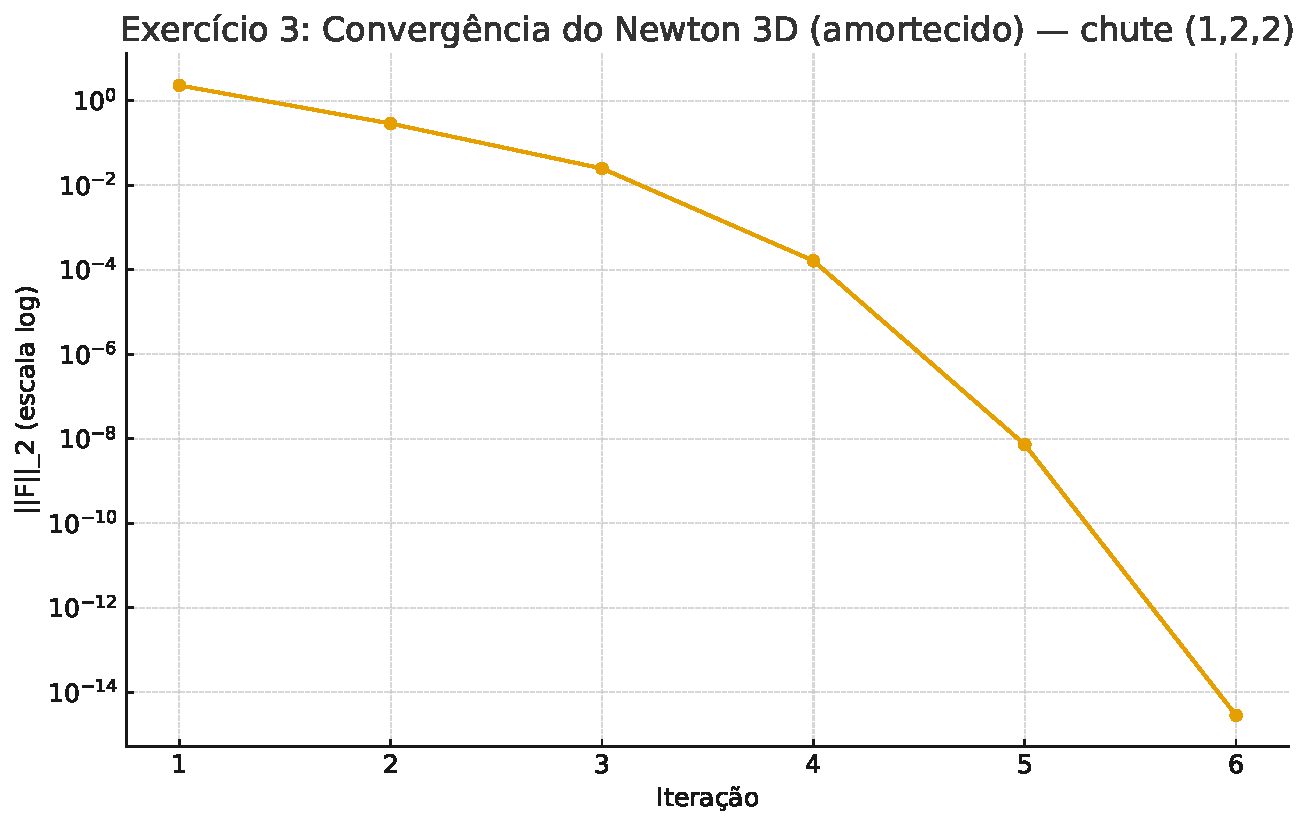
\includegraphics[width=0.75\textwidth]{figures/ex3_convergence_normF.pdf}
  \caption{Convergência de $\|F\|_2$ (Newton 3D amortecido) a partir de $(1,2,2)$.}
  \label{fig:ex3_normF}
\end{figure}

\begin{figure}[H]
  \centering
  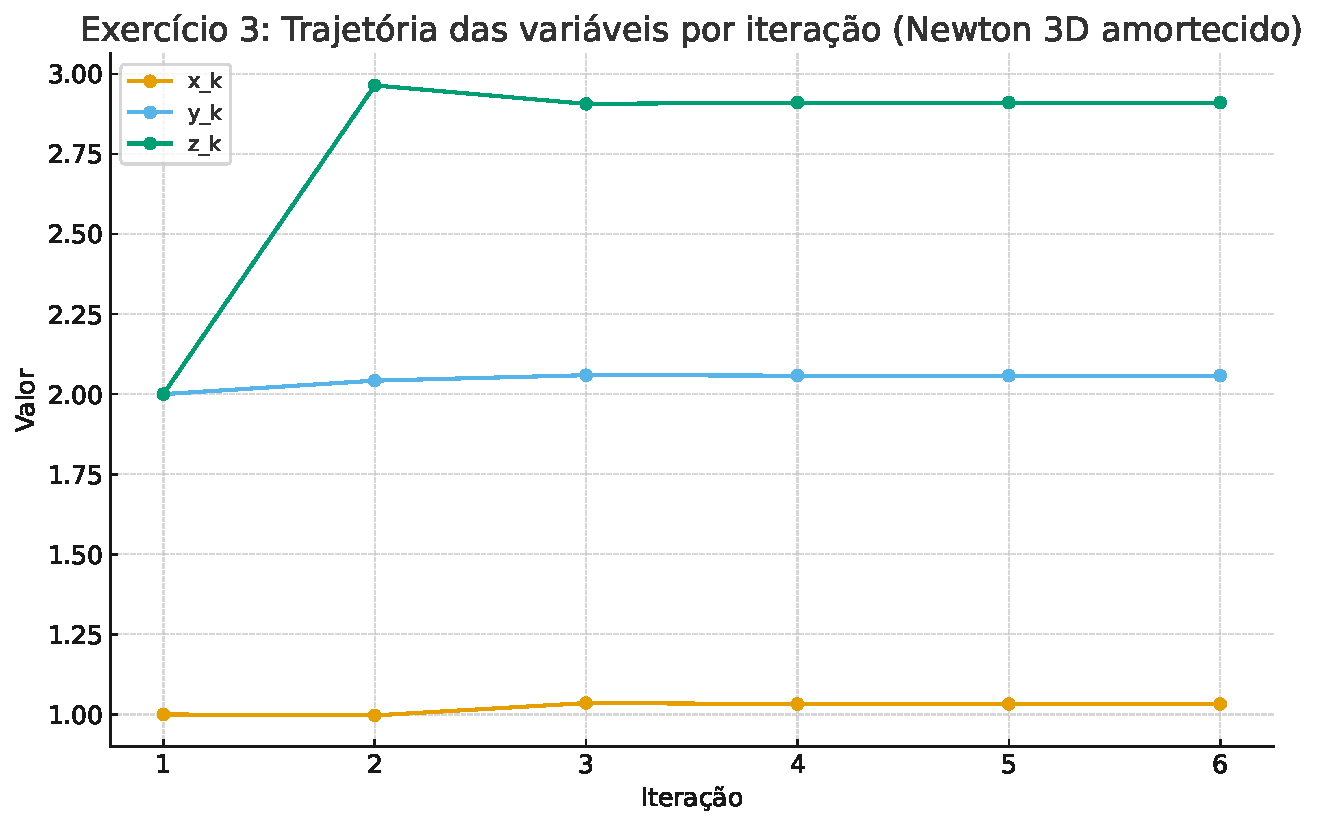
\includegraphics[width=0.8\textwidth]{figures/ex3_state_trajectory.pdf}
  \caption{Trajetória de $(x_k,y_k,z_k)$ por iteração (Newton 3D amortecido).}
  \label{fig:ex3_state}
\end{figure}

\begin{table}[H]
\centering
\caption{Comparação entre Newton 3D (puro e amortecido) e \texttt{fsolve} (Ex.3).}
\label{tab:ex3_methods}
\begin{tabular}{l r r r r r r r}
\hline
Método & $x_0$ & $y_0$ & $z_0$ & $x$ & $y$ & $z$ & $\|F\|_2$ \\
\hline
Newton-3D (damped) & 1.00 & 2.00 & 2.00 & 1.032548 & 2.057768 & 2.910139 & 2.844e-15 \\
Newton-3D (pure) & 1.00 & 2.00 & 2.00 & 1.032548 & 2.057768 & 2.910139 & 2.844e-15 \\
Newton-3D (damped) & 0.80 & 1.80 & 2.00 & 0.730519 & 1.403044 & 4.235598 & 4.886e-14 \\
Newton-3D (pure) & 0.80 & 1.80 & 2.00 & 0.730519 & 1.403044 & 4.235598 & 9.930e-16 \\
Newton-3D (damped) & 1.20 & 2.20 & 2.00 & 1.032548 & 2.057768 & 2.910139 & 1.018e-15 \\
Newton-3D (pure) & 1.20 & 2.20 & 2.00 & 1.032548 & 2.057768 & 2.910139 & 1.018e-15 \\
Newton-3D (damped) & 1.00 & 2.00 & 2.20 & 1.032548 & 2.057768 & 2.910139 & 1.018e-15 \\
Newton-3D (pure) & 1.00 & 2.00 & 2.20 & 1.032548 & 2.057768 & 2.910139 & 1.018e-15 \\
Newton-3D (damped) & 1.00 & 2.00 & 1.80 & 1.032548 & 2.057768 & 2.910139 & 4.619e-13 \\
Newton-3D (pure) & 1.00 & 2.00 & 1.80 & 1.032548 & 2.057768 & 2.910139 & 4.619e-13 \\
fsolve & 1.00 & 2.00 & 2.00 & 1.032548 & 2.057768 & 2.910139 & 2.844e-15 \\
\hline
\end{tabular}
\end{table}

\subsection{Conclusão.}
O sistema 3D é não linear e acoplado; o \textbf{Newton 3D amortecido} apresentou convergência robusta a partir de chutes próximos de $(1,2,2)$, enquanto o \textbf{Newton puro} foi mais sensível ao passo. O \textbf{\texttt{fsolve}} mostrou-se consistente (quando disponível), mas com maior custo por avaliação. As trajetórias e o decaimento de $\|F\|_2$ sustentam a correção numérica e a estabilidade do método.

\subsection{Implementação}
\label{subsec:ex3-implementacao}

\paragraph{Visão geral.}
O código do Exercício~3 implementa a solução de um \textbf{sistema não linear tridimensional} composto por três equações acopladas:
\[
\begin{cases}
\sin(xy) + e^{-xz} - 0.9 = 0,\\
z\sqrt{x^2 + y^2} - 6.7 = 0,\\
\tan\!\left(\dfrac{y}{x}\right) + \cos(z) + 3.2 = 0.
\end{cases}
\]
O objetivo é determinar \((x, y, z)\) que anule simultaneamente \(F(x,y,z)\).
O método principal é o \textbf{Newton–Jacobian 3D}, em versões \emph{pura} e \emph{amortecida}, comparado também com a solução via \textbf{\texttt{fsolve}} (SciPy) para validar robustez e precisão.

\paragraph{Arquitetura das funções.}
\begin{description}
  \item[\texttt{F(v)}]
  Retorna o vetor de funções não lineares \(F(x,y,z)=[f_1,f_2,f_3]^T\), onde:
  \begin{align*}
  f_1 &= \sin(xy) + e^{-xz} - 0.9,\\
  f_2 &= z\sqrt{x^2 + y^2} - 6.7,\\
  f_3 &= \tan(y/x) + \cos(z) + 3.2.
  \end{align*}
  Essa função é usada para avaliar o resíduo \(\|F(x_k,y_k,z_k)\|_2\) a cada iteração.

  \item[\texttt{J(v)}]
  Calcula o \textbf{Jacobiano completo} do sistema:
  \[
  J(x,y,z)=
  \begin{bmatrix}
  \cos(xy)y - z e^{-xz} & \cos(xy)x & -x e^{-xz}\\
  z\frac{x}{r} & z\frac{y}{r} & r\\
  -\dfrac{y}{x^2}\sec^2\!\left(\tfrac{y}{x}\right) & \dfrac{1}{x}\sec^2\!\left(\tfrac{y}{x}\right) & -\sin(z)
  \end{bmatrix}, \quad r=\sqrt{x^2+y^2}.
  \]
  Cada derivada parcial foi obtida analiticamente. Essa matriz é usada para resolver o sistema linear de correção de Newton \(J\,\Delta z=-F\).

  \item[\texttt{newton3d(x0, tol, maxit, damping)}]
  Implementa o método iterativo de Newton 3D:
  \begin{itemize}
    \item \textbf{Entrada:} chute inicial \(x_0,y_0,z_0\), tolerância \texttt{tol}, máximo de iterações \texttt{maxit}, flag \texttt{damping} (para ativar o amortecimento).
    \item \textbf{Passos principais:}
      \begin{enumerate}
        \item Avaliar \(F(x_k,y_k,z_k)\) e \(J(x_k,y_k,z_k)\);
        \item Resolver \(J\,\Delta = -F\);
        \item Atualizar \(x_{k+1},y_{k+1},z_{k+1} = x_k,y_k,z_k + \alpha\,\Delta\), onde \(\alpha \in (0,1]\);
        \item Parar quando \(\|F(x_{k+1},y_{k+1},z_{k+1})\|_2 < \texttt{tol}\).
      \end{enumerate}
    \item \textbf{Amortecimento (backtracking):} o fator \(\alpha\) é reduzido iterativamente até que \(\|F(x_{k+1})\|_2 < \|F(x_k)\|_2\), garantindo convergência mesmo quando o chute inicial é distante.
    \item \textbf{Saída:} vetor solução \((x,y,z)\), número de iterações, flag de convergência e histórico de iterações.
  \end{itemize}

  \item[\texttt{fsolve(F, x0)}]
  Resolve o mesmo sistema usando a rotina da biblioteca \texttt{SciPy}.
  Internamente, o \texttt{fsolve} combina o método de Newton com estratégias de \emph{região de confiança} e ajustes de passo (Levenberg–Marquardt ou dogleg). 
  Embora mais custoso, ele é menos propenso a divergência.

  \item[\texttt{main()}]
  Coordena toda a execução:
  \begin{enumerate}
    \item Define múltiplos chutes iniciais próximos de $(1,2,2)$;
    \item Executa o Newton puro e amortecido para cada chute;
    \item (Opcional) Executa \texttt{fsolve} para comparação;
    \item Armazena resultados em \texttt{tables/ex3\_3d\_newton\_vs\_fsolve\_results.csv};
    \item Gera figuras:
      \begin{itemize}
        \item \texttt{ex3\_convergence\_normF.pdf} — decaimento de $\|F\|_2$ por iteração;
        \item \texttt{ex3\_state\_trajectory.pdf} — evolução de $(x_k,y_k,z_k)$ ao longo das iterações.
      \end{itemize}
  \end{enumerate}
\end{description}

\paragraph{Critérios numéricos.}
Adotou-se \(\texttt{tol}=10^{-10}\) e \(\texttt{maxit}=100\).
A convergência é avaliada pela norma Euclidiana \(\|F\|_2\).
O amortecimento (\emph{backtracking}) assegura que o resíduo diminua monotonicamente.

\paragraph{Diferenças observadas entre métodos.}
O \textbf{Newton puro} converge mais rapidamente quando o chute está próximo da raiz, mas pode divergir para regiões onde o Jacobiano é mal condicionado.
O \textbf{Newton amortecido} sacrifica velocidade em prol da robustez global, sendo capaz de corrigir trajetórias divergentes.
O \textbf{\texttt{fsolve}} é o mais robusto — sua estratégia adaptativa evita divergência, mas exige mais avaliações de função e derivadas.

\paragraph{Referência ao código completo.}
O código integral correspondente encontra-se no \textbf{Apêndice} (ver \emph{Exercício 3 — Sistema 3D: Newton--Jacobian e \texttt{fsolve}}),
importado diretamente via:
\texttt{\textbackslash inputminted[fontsize=\footnotesize,breaklines]\{python\}\{code/ex3\_newton3d\_vs\_fsolve.py\}}.


\section{Glossário de Variáveis}
\addcontentsline{toc}{section}{Glossário de Variáveis}

\begin{description}
    \item[$x,\,y,\,z$] Variáveis independentes do sistema ou da função. 
    No Ex.~1, $x$ é a variável espacial no domínio $[-1,1]$; 
    nos Exs.~2 e 3, representam incógnitas do sistema não linear.

    \item[$y(x)$] Função dependente de $x$ (Ex.~1), solução da EDO $y'' = e^{y}$.

    \item[$y',\,y''$] Primeira e segunda derivadas de $y(x)$ em relação a $x$,
    aproximadas numericamente pelas matrizes diferenciais de Chebyshev $D$ e $D^2$.

    \item[$D,\,D^2$] Matrizes diferenciais de Chebyshev: $D$ representa a derivada de primeira ordem e $D^2$ a segunda ordem, 
    construídas a partir dos nós de Chebyshev–Lobatto.

    \item[$R(x)$] Resíduo do problema diferencial (Ex.~1), definido como $R(x) = y'' - e^{y}$.

    \item[$R'(x)$] Derivada do resíduo, usada para verificar suavidade e estabilidade da solução espectral.

    \item[$J$] Matriz Jacobiana, que contém as derivadas parciais das funções não lineares em relação às variáveis.
    É usada nos métodos de Newton para resolver sistemas do tipo $J \Delta z = -F(z)$.

    \item[$F$] Vetor de funções não lineares:
    \begin{itemize}
        \item No Ex.~1, $F(y) = D^2 y - e^{y}$.
        \item No Ex.~2, $F(x,y) = [x^3 + y - 1,\; y^3 - x + 1]^T$.
        \item No Ex.~3, $F(x,y,z) = [\sin(xy) + e^{-xz} - 0.9,\; z\sqrt{x^2 + y^2} - 6.7,\; \tan(y/x) + \cos(z) + 3.2]^T$.
    \end{itemize}

    \item[$\Delta y$, $\Delta z$] Vetores de correção obtidos em cada iteração de Newton, solução de $J \Delta = -F$.

    \item[$\alpha$] Fator de amortecimento (\emph{damping}) no método de Newton amortecido.
    Multiplica o passo $\Delta z$ para garantir decréscimo de $\|F(z_{k+1})\|$ e evitar divergência.

    \item[$\|F\|_2$] Norma Euclidiana do vetor $F$, usada como métrica de erro para avaliar a convergência.

    \item[$N$] Número de subintervalos (ou grau do polinômio) na discretização de Chebyshev; o número total de nós é $N{+}1$.

    \item[$M$] Número de pontos da malha fina usada para comparação entre soluções interpoladas no estudo de refinamento (Ex.~1).

    \item[$\|\Delta y\|_{\infty}$] Norma máxima da correção $\Delta y$ no método de Newton, usada como critério de parada.

    \item[$\tan$, $\sin$, $\cos$, $\exp$] Funções trigonométricas e exponencial, aplicadas ponto a ponto no cálculo das funções e derivadas.

    \item[$f_1,\,f_2,\,f_3$] Equações componentes do sistema não linear (Ex.~2 e Ex.~3).

    \item[$\texttt{fsolve}$] Função da biblioteca SciPy que resolve sistemas não lineares
    via métodos híbridos (Newton + região de confiança), com controle automático de passo.

    \item[$\text{tol}$] Tolerância numérica, usada como limite de erro para o critério de convergência.

    \item[$\text{maxit}$] Número máximo de iterações permitidas no processo iterativo.

    \item[$\text{hist}$] Histórico de iterações armazenando valores intermediários das variáveis e da norma do resíduo em cada passo.
\end{description}


\appendix
\section{Códigos Completos}

\subsection{Exercício 1 — Colocalização de Chebyshev e Método de Newton}
\inputminted[fontsize=\footnotesize,breaklines]{python}{code/ex1_cheb_newton.py}

\subsection{Exercício 2 — Sistema Não Linear: Newton--Jacobian e \texttt{fsolve}}
\inputminted[fontsize=\footnotesize,breaklines]{python}{code/ex2_newton_vs_fsolve.py}

\subsection{Exercício 3 — Sistema 3D: Newton--Jacobian e \texttt{fsolve}}
\inputminted[fontsize=\footnotesize,breaklines]{python}{code/ex3_newton3d_vs_fsolve.py}

\section{Setup ambiente Python}
\addcontentsline{toc}{section}{Instruções para Configuração do Ambiente Python}

\paragraph{Versão da linguagem.}
Os experimentos foram desenvolvidos e testados em:
\begin{itemize}
  \item \textbf{Python:} 3.12.10 (64 bits)
  \item \textbf{Sistema operacional:} Linux (WSL2) / compatível com Windows, macOS e distribuições baseadas em Debian.
\end{itemize}

\paragraph{Dependências principais.}
A seguir listam-se os pacotes necessários e suas respectivas versões utilizadas durante os experimentos:

\begin{table}[H]
\centering
\caption{Pacotes e versões utilizados nos exercícios.}
\begin{tabular}{l l}
\hline
\textbf{Biblioteca} & \textbf{Versão recomendada} \\
\hline
\texttt{numpy} & 1.26.0 \\
\texttt{scipy} & 1.14.1 \\
\texttt{pandas} & 2.2.2 \\
\texttt{matplotlib} & 3.9.2 \\
\texttt{minted} (para LaTeX) & 2.9 \\
\texttt{Pygments} (para sintaxe colorida no LaTeX) & 2.18.0 \\
\texttt{python3-tk} (opcional, para gráficos locais) & -- \\
\hline
\end{tabular}
\end{table}

\paragraph{Criação do ambiente virtual.}
Para garantir a reprodutibilidade, recomenda-se criar um ambiente virtual isolado:

\begin{minted}[fontsize=\footnotesize,breaklines]{bash}
# Criar o ambiente virtual
python3 -m venv venv

# Ativar o ambiente (Linux/Mac)
source venv/bin/activate

# Ativar o ambiente (Windows)
venv\Scripts\activate
\end{minted}

\paragraph{Instalação das dependências.}
Após ativar o ambiente, instalar os pacotes requeridos:

\begin{minted}[fontsize=\footnotesize,breaklines]{bash}
pip install numpy==1.26.0 scipy==1.14.1 pandas==2.2.2 matplotlib==3.9.2
\end{minted}

\paragraph{Estrutura esperada do projeto.}
Após a configuração, a estrutura de diretórios deve ser:

\begin{verbatim}
PTC5725_Tarefa04/
├── code/
│   ├── ex1_cheb_newton.py
│   ├── ex2_newton_vs_fsolve.py
│   └── ex3_newton3d_vs_fsolve.py
├── figures/
├── tables/
├── refs/
│   └── refs.bib
└── main.tex
\end{verbatim}

\paragraph{Execução dos scripts.}
Cada script Python pode ser executado individualmente para gerar suas figuras e tabelas:

\begin{minted}[fontsize=\footnotesize,breaklines]{bash}
# Executar o exercício 1
python code/ex1_cheb_newton.py

# Executar o exercício 2
python code/ex2_newton_vs_fsolve.py

# Executar o exercício 3
python code/ex3_newton3d_vs_fsolve.py
\end{minted}

As saídas (figuras e tabelas) são automaticamente salvas nas pastas correspondentes.  
Após gerar todas as saídas, o relatório pode ser compilado com \LaTeX:

\begin{minted}[fontsize=\footnotesize,breaklines]{bash}
pdflatex main.tex
bibtex main
pdflatex main.tex
pdflatex main.tex
\end{minted}

% ---------------- Referências ----------------
\bibliographystyle{plain}
\bibliography{refs/refs}
\end{document}
